\documentclass{beamer}
\usepackage{tikz}
\usetikzlibrary{positioning, arrows.meta, shadows, shapes, arrows, fit}
\usetheme{Madrid}

\title{EcoSenseNet - Smart Environment Prediction and Alert System}
\author{Pratiksha}
\institute{Indian Institute of Information Technology Senapati, Manipur}
\date{\today}

\begin{document}

\frame{\titlepage}

\begin{frame}{Outline}
  \tableofcontents
\end{frame}

\section{Introduction, Objective \& Contribution}
\begin{frame}{Introduction, Objective \& Contribution}
  \begin{block}{Introduction}
    EcoSenseNet is a smart environment prediction and alert system designed for localized areas like a college campus. It integrates IoT sensors, machine learning, and offline communication to deliver real-time environmental predictions and alerts, especially when the internet is unavailable.
  \end{block}
  \begin{block}{Objectives}
    \begin{itemize}
      \item To acquire real-time environmental data using various sensors.
      \item To process and predict environmental trends using a locally deployed LSTM model.
      \item To enable completely offline alert distribution using Reticulum MeshChat over LoRa and Wi-Fi.
      \item To provide an additional chat interface for administrators and students to communicate during outages.
    \end{itemize}
  \end{block}
  \begin{block}{Contribution}
    A fully functional, end-to-end offline environmental monitoring system that seamlessly integrates IoT sensing, local machine learning inference, and mesh-based data broadcasting. It provides a scalable and affordable solution for rural or disaster-response networks.
  \end{block}
\end{frame}

\section{Background / Existing Work}
\begin{frame}{Background / Existing Work}
  \begin{block}{Existing Work}
    \begin{itemize}
      \item Most environmental monitoring systems rely on constant internet connectivity and cloud-based analytics.
      \item Technologies like Wi-Fi and GSM have limitations in terms of range, power consumption, and reliability during disasters.
      \item Existing LoRa networks are often dependent on cloud-connected gateways.
    \end{itemize}
  \end{block}
  \begin{block}{Problems in Existing Work}
    \begin{itemize}
      \item \textbf{Network Dependence:} Systems fail without internet access.
      \item \textbf{Centralized Architecture:} Single points of failure (gateways, cloud servers).
      \item \textbf{Lack of Edge Intelligence:} Few systems perform predictive ML locally.
    \end{itemize}
  \end{block}
  \begin{block}{How Our Project Overcomes These Problems}
    EcoSenseNet uses a decentralized, offline-first approach. It combines local data processing with a LoRa-based mesh network, eliminating the need for internet or cloud services. The system's on-device LSTM model provides predictive capabilities at the edge, ensuring continuous operation even in disconnected environments.
  \end{block}
\end{frame}

\section{Proposed System / Architecture}
\begin{frame}{Proposed System / Architecture}
  \begin{columns}
    \begin{column}{0.5\textwidth}
      \begin{figure}
        \centering
        \resizebox{1\textwidth}{!}{
        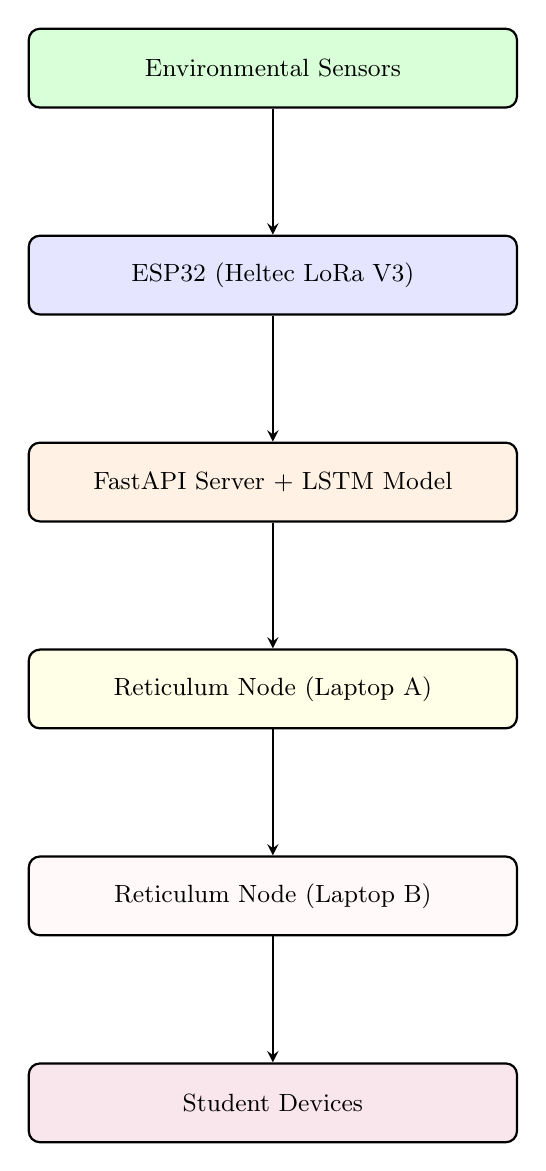
\begin{tikzpicture}[
            font=\small,
            >=stealth,
            node distance=1.6cm,
            box/.style={rectangle, draw, rounded corners, minimum width=6.2cm, minimum height=1.0cm, align=center, thick, fill=blue!5},
            arrow/.style={->, thick, >=stealth}
        ]
        \node[box, fill=green!15] (sensors) {Environmental Sensors};
        \node[box, fill=blue!10, below=of sensors] (esp32) {ESP32 (Heltec LoRa V3)};
        \node[box, fill=orange!10, below=of esp32] (fastapi) {FastAPI Server + LSTM Model};
        \node[box, fill=yellow!10, below=of fastapi] (reticA) {Reticulum Node (Laptop A)};
        \node[box, fill=pink!10, below=of reticA] (reticB) {Reticulum Node (Laptop B)};
        \node[box, fill=purple!10, below=of reticB] (users) {Student Devices};
        \draw[arrow] (sensors) -- (esp32);
        \draw[arrow] (esp32) -- (fastapi);
        \draw[arrow] (fastapi) -- (reticA);
        \draw[arrow] (reticA) -- (reticB);
        \draw[arrow] (reticB) -- (users);
        \end{tikzpicture}
        }
        \caption{System Architecture}
      \end{figure}
    \end{column}
    \begin{column}{0.5\textwidth}
      \begin{block}{Process}
        \begin{enumerate}
          \item \textbf{Input:} Real-time environmental data is collected by sensors connected to an ESP32.
          \item \textbf{Process:} The data is sent to a local FastAPI server, which uses an LSTM model to predict environmental trends for the next 3 hours.
          \item \textbf{Output:} The predictions and any alerts are broadcasted over a LoRa-based mesh network to other devices.
        \end{enumerate}
      \end{block}
      \begin{block}{Tools Used}
        \begin{itemize}
          \item \textbf{Hardware:} ESP32, Heltec LoRa V3, MQ-series sensors, DHT22.
          \item \textbf{Software:} FastAPI, TensorFlow, Reticulum, Arduino.
          \item \textbf{Languages:} Python, C++.
        \end{itemize}
      \end{block}
    \end{column}
  \end{columns}
\end{frame}

\section{Result \& Analysis}
\begin{frame}{Result \& Analysis}
  \begin{block}{Testing}
    The system was tested within the IIIT Manipur campus. Two laptops were used: one as a base station with sensors, and the other as a receiving node at various distances. The tests were conducted without any internet connectivity.
  \end{block}
  \begin{block}{Key Results}
    \begin{table}
      \centering
      \caption{System Performance}
      \begin{tabular}{|l|l|}
        \hline
        \textbf{Metric} & \textbf{Result} \\
        \hline
        End-to-End Latency & 4-7 seconds \\
        \hline
        LSTM Prediction Time & 150-250 ms \\
        \hline
        LoRa Reliability (500m) & 92-95\% \\
        \hline
        LoRa Reliability (800m) & ~85\% \\
        \hline
        False Alert Rate & ~8\% \\
        \hline
      \end{tabular}
    \end{table}
  \end{block}
  \begin{block}{Analysis}
    The results show that the system can reliably collect, process, and transmit environmental data and alerts in an offline setting. The latency is low enough for real-time emergency notifications, and the LoRa network provides good coverage across the campus.
  \end{block}
\end{frame}

\section{Conclusion}
\begin{frame}{Conclusion}
  \begin{block}{Summary}
    We have successfully developed EcoSenseNet, a decentralized and offline-first environmental monitoring and alert system. The system combines IoT, machine learning, and mesh networking to provide a resilient and low-cost solution for disaster-prone areas.
  \end{block}
  \begin{block}{Achievements}
    \begin{itemize}
      \item Achieved reliable end-to-end functionality, from data collection to alert delivery.
      \item The system operates with low latency (4-7 seconds) and high prediction accuracy (>87\%).
      \item Demonstrated the feasibility of a fully offline communication system for emergency scenarios.
    \end{itemize}
  \end{block}
  \begin{block}{Future Enhancements}
    \begin{itemize}
      \item Replace laptops with Raspberry Pi for lower power consumption and a smaller form factor.
      \item Develop a mobile application for a more user-friendly interface and push notifications.
      \item Add more sensors and improve the machine learning model for greater accuracy and a wider range of applications.
    \end{itemize}
  \end{block}
\end{frame}

\end{document}
